\documentclass[14pt]{extbook}
\usepackage{multicol, enumerate, enumitem, hyperref, color, soul, setspace, parskip, fancyhdr} %General Packages
\usepackage{amssymb, amsthm, amsmath, bbm, latexsym, units, mathtools} %Math Packages
\everymath{\displaystyle} %All math in Display Style
% Packages with additional options
\usepackage[headsep=0.5cm,headheight=12pt, left=1 in,right= 1 in,top= 1 in,bottom= 1 in]{geometry}
\usepackage[usenames,dvipsnames]{xcolor}
\usepackage{dashrule}  % Package to use the command below to create lines between items
\newcommand{\litem}[1]{\item#1\hspace*{-1cm}\rule{\textwidth}{0.4pt}}
\pagestyle{fancy}
\lhead{Progress Quiz 3}
\chead{}
\rhead{Version B}
\lfoot{}
\cfoot{}
\rfoot{Fall 2020}
\begin{document}

\begin{enumerate}
\litem{
Describe the end behavior of the polynomial below.\[ f(x) = 6(x + 6)^{5}(x - 6)^{6}(x + 2)^{2}(x - 2)^{3} \]\begin{enumerate}[label=\Alph*.]
\begin{multicols}{2}\item 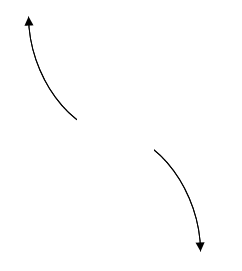
\includegraphics[width = 0.3\textwidth]{../Figures/polyEndBehaviorCopyAB.png}\item 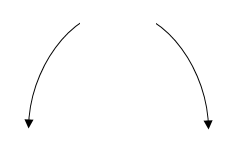
\includegraphics[width = 0.3\textwidth]{../Figures/polyEndBehaviorCopyBB.png}\item 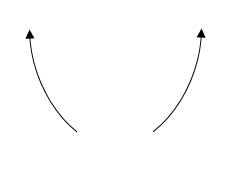
\includegraphics[width = 0.3\textwidth]{../Figures/polyEndBehaviorCopyCB.png}\item 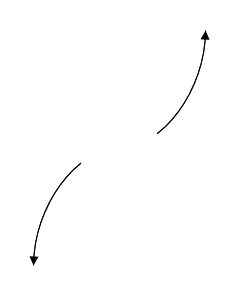
\includegraphics[width = 0.3\textwidth]{../Figures/polyEndBehaviorCopyDB.png}\end{multicols}\item None of the above.
\end{enumerate} }
\litem{
Describe the end behavior of the polynomial below.\[ f(x) = 2(x - 7)^{3}(x + 7)^{6}(x + 3)^{3}(x - 3)^{3} \]\begin{enumerate}[label=\Alph*.]
\begin{multicols}{2}\item 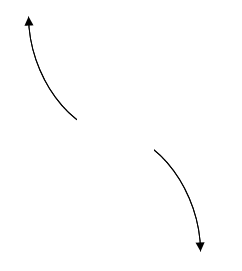
\includegraphics[width = 0.3\textwidth]{../Figures/polyEndBehaviorAB.png}\item 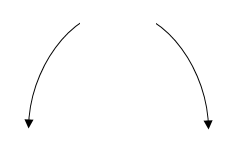
\includegraphics[width = 0.3\textwidth]{../Figures/polyEndBehaviorBB.png}\item 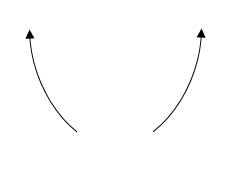
\includegraphics[width = 0.3\textwidth]{../Figures/polyEndBehaviorCB.png}\item 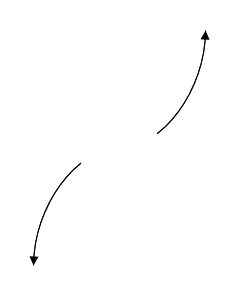
\includegraphics[width = 0.3\textwidth]{../Figures/polyEndBehaviorDB.png}\end{multicols}\item None of the above.
\end{enumerate} }
\litem{
Construct the lowest-degree polynomial given the zeros below. Then, choose the intervals that contain the coefficients of the polynomial in the form $ax^3+bx^2+cx+d$.\[ \frac{-7}{4}, 3, \text{ and } \frac{-1}{3} \]\begin{enumerate}[label=\Alph*.]
\item \( a \in [11, 19], b \in [-11, -6], c \in [-71, -67], \text{ and } d \in [-22, -17] \)
\item \( a \in [11, 19], b \in [-63, -49], c \in [42, 47], \text{ and } d \in [9, 23] \)
\item \( a \in [11, 19], b \in [18, 26], c \in [-61, -54], \text{ and } d \in [-22, -17] \)
\item \( a \in [11, 19], b \in [-11, -6], c \in [-71, -67], \text{ and } d \in [9, 23] \)
\item \( a \in [11, 19], b \in [7, 17], c \in [-71, -67], \text{ and } d \in [9, 23] \)

\end{enumerate} }
\litem{
Construct the lowest-degree polynomial given the zeros below. Then, choose the intervals that contain the coefficients of the polynomial in the form $x^3+bx^2+cx+d$.\[ -3 - 2 i \text{ and } -4 \]\begin{enumerate}[label=\Alph*.]
\item \( b \in [6, 17], c \in [35.32, 37.41], \text{ and } d \in [48.7, 52.2] \)
\item \( b \in [-6, 4], c \in [6.42, 8.44], \text{ and } d \in [10.6, 15.5] \)
\item \( b \in [-11, -5], c \in [35.32, 37.41], \text{ and } d \in [-52.5, -50.6] \)
\item \( b \in [-6, 4], c \in [5.93, 6.06], \text{ and } d \in [6.6, 10.2] \)
\item \( \text{None of the above.} \)

\end{enumerate} }
\litem{
Construct the lowest-degree polynomial given the zeros below. Then, choose the intervals that contain the coefficients of the polynomial in the form $ax^3+bx^2+cx+d$.\[ \frac{1}{4}, 4, \text{ and } 7 \]\begin{enumerate}[label=\Alph*.]
\item \( a \in [2, 5], b \in [-47.3, -43.3], c \in [123, 132], \text{ and } d \in [23, 29] \)
\item \( a \in [2, 5], b \in [-12.4, -9.4], c \in [-115, -111], \text{ and } d \in [-31, -19] \)
\item \( a \in [2, 5], b \in [-47.3, -43.3], c \in [123, 132], \text{ and } d \in [-31, -19] \)
\item \( a \in [2, 5], b \in [43.4, 45.2], c \in [123, 132], \text{ and } d \in [23, 29] \)
\item \( a \in [2, 5], b \in [-43.9, -40.8], c \in [100, 102], \text{ and } d \in [23, 29] \)

\end{enumerate} }
\litem{
Which of the following equations \textit{could} be of the graph presented below?
\begin{center}
    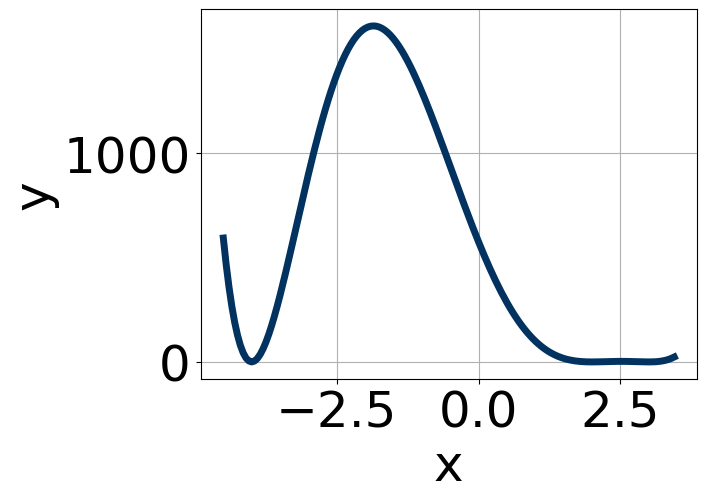
\includegraphics[width=0.5\textwidth]{../Figures/polyGraphToFunctionCopyB.png}
\end{center}
\begin{enumerate}[label=\Alph*.]
\item \( 4(x - 2)^{6} (x + 4)^{4} (x - 3)^{6} \)
\item \( -12(x - 2)^{8} (x + 4)^{6} (x - 3)^{7} \)
\item \( 14(x - 2)^{8} (x + 4)^{8} (x - 3)^{11} \)
\item \( -4(x - 2)^{4} (x + 4)^{4} (x - 3)^{8} \)
\item \( 18(x - 2)^{6} (x + 4)^{11} (x - 3)^{9} \)

\end{enumerate} }
\litem{
Which of the following equations \textit{could} be of the graph presented below?
\begin{center}
    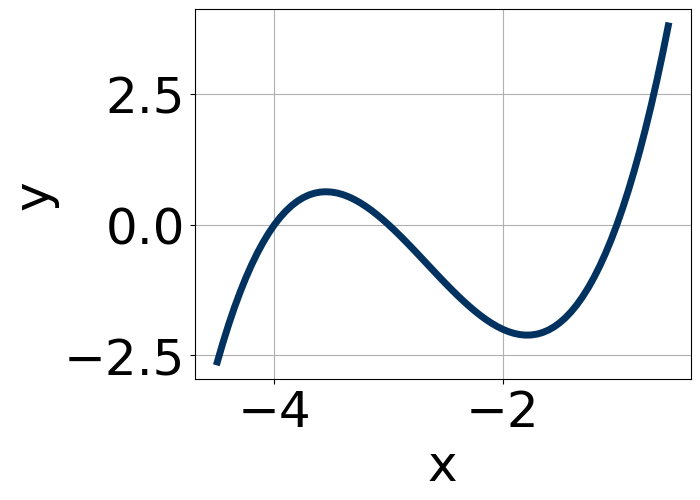
\includegraphics[width=0.5\textwidth]{../Figures/polyGraphToFunctionB.png}
\end{center}
\begin{enumerate}[label=\Alph*.]
\item \( -17(x + 4)^{9} (x + 1)^{11} (x + 3)^{5} \)
\item \( 20(x + 4)^{11} (x + 1)^{11} (x + 3)^{11} \)
\item \( 16(x + 4)^{10} (x + 1)^{4} (x + 3)^{7} \)
\item \( 2(x + 4)^{6} (x + 1)^{5} (x + 3)^{9} \)
\item \( -5(x + 4)^{4} (x + 1)^{5} (x + 3)^{11} \)

\end{enumerate} }
\litem{
Construct the lowest-degree polynomial given the zeros below. Then, choose the intervals that contain the coefficients of the polynomial in the form $x^3+bx^2+cx+d$.\[ 5 + 3 i \text{ and } -1 \]\begin{enumerate}[label=\Alph*.]
\item \( b \in [-6, 5], c \in [-9, -3], \text{ and } d \in [-8, -4.4] \)
\item \( b \in [-6, 5], c \in [-3, 5], \text{ and } d \in [-4.4, -2.5] \)
\item \( b \in [8, 12], c \in [20, 27], \text{ and } d \in [-36.8, -29.5] \)
\item \( b \in [-16, -5], c \in [20, 27], \text{ and } d \in [31.3, 34.5] \)
\item \( \text{None of the above.} \)

\end{enumerate} }
\litem{
Describe the zero behavior of the zero $x = -7$ of the polynomial below.\[ f(x) = 7(x + 7)^{4}(x - 7)^{7}(x + 3)^{5}(x - 3)^{7} \]\begin{enumerate}[label=\Alph*.]
\begin{multicols}{2}\item 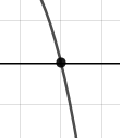
\includegraphics[width = 0.3\textwidth]{../Figures/polyZeroBehaviorCopyAB.png}\item 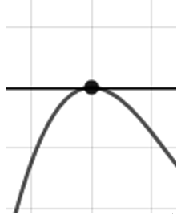
\includegraphics[width = 0.3\textwidth]{../Figures/polyZeroBehaviorCopyBB.png}\item 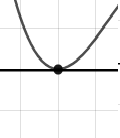
\includegraphics[width = 0.3\textwidth]{../Figures/polyZeroBehaviorCopyCB.png}\item 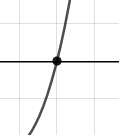
\includegraphics[width = 0.3\textwidth]{../Figures/polyZeroBehaviorCopyDB.png}\end{multicols}\item None of the above.
\end{enumerate} }
\litem{
Describe the zero behavior of the zero $x = -3$ of the polynomial below.\[ f(x) = 5(x - 3)^{7}(x + 3)^{10}(x + 6)^{4}(x - 6)^{8} \]\begin{enumerate}[label=\Alph*.]
\begin{multicols}{2}\item 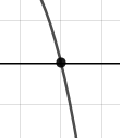
\includegraphics[width = 0.3\textwidth]{../Figures/polyZeroBehaviorAB.png}\item 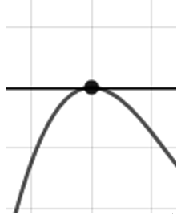
\includegraphics[width = 0.3\textwidth]{../Figures/polyZeroBehaviorBB.png}\item 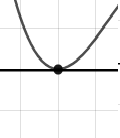
\includegraphics[width = 0.3\textwidth]{../Figures/polyZeroBehaviorCB.png}\item 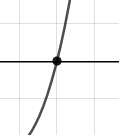
\includegraphics[width = 0.3\textwidth]{../Figures/polyZeroBehaviorDB.png}\end{multicols}\item None of the above.
\end{enumerate} }
\end{enumerate}

\end{document}